% Insertable section synthesizing the mechanistic decomposition of the late commitment lever.
% % Insertable section synthesizing the mechanistic decomposition of the late commitment lever.
% % Insertable section synthesizing the mechanistic decomposition of the late commitment lever.
% % Insertable section synthesizing the mechanistic decomposition of the late commitment lever.
% \input{section_mechanism} after \S\ref{sec:xmodel} (cross-architecture), before Discussion.
% Requires bib keys: geva, induction, mathframework, ioi (entries listed at the end of this file).

\section{Opening the lever: a sparse attention-head circuit}\label{sec:decomp}
The lever is a single late-layer residual patch; we now open it. Because a pre-norm block writes its output as
an \emph{exact} sum, $y_L = x_L + a_L + m_L$ (input residual, attention contribution, MLP contribution), the
published donor patch $\Delta_{\text{full}} = y^{\text{donor}}_L - y^{\text{point}}_L = \Delta x + \Delta a +
\Delta m$ is exactly additive in the residual. We therefore re-inject each component alone with an additive hook
at the layer-$L$ output and read the one-token $\Delta P(\text{edit})$, the same metric as the dense profile of
\S\ref{sec:stats}. Two gates hold throughout: the additive split reconstructs the captured residual to relative
error $0.0025$ (L55) / $0.0024$ (L59), and the \texttt{full} re-injection reproduces the published lever exactly
(elicit emission $0.23\!\to\!0.77$@L59, brake $0.48\!\to\!0.03$@L55), so the decomposition measures the same
intervention. All numbers are $n{=}60$/condition on Qwen3.6-27B.

\paragraph{Attention writes the elicit; the MLP is inert; the brake is distributed.}
Table~\ref{tab:decomp} gives the recovery fraction $r = \Delta P_{\text{comp}}/\Delta P_{\text{full}}$ of each
component. The two directions decompose \emph{differently}. For the \textbf{elicit}, the L59 attention sublayer
is the single largest writer ($r_{\text{attn}}{=}0.43$, 95\% CI $[0.33,0.53]$), the \textbf{MLP is null}
($r_{\text{mlp}}{=}{-}0.04$; paired Wilcoxon attn$\gg$mlp $p{=}1.8\mathrm{e}{-}8$), and the attention write is
\emph{direction-specific} (task-matched $\Delta P{=}{+}0.223$ vs.\ random-donor $+0.100$, $2.2\times$); under
generation the attention component alone roughly doubles emission ($0.23\!\to\!0.45$) while the MLP component is
inert ($0.25$). At L55 neither sublayer writes the signal --- it is still \emph{arriving} via the residual from
below ($r_{\text{inp}}{=}0.52$) --- so the attention write fires specifically at L59. The \textbf{brake} localizes
to \emph{neither} sublayer ($r_{\text{attn}},r_{\text{mlp}}\!\approx\!0$ at both layers); $\sim$35--40\% is
carried by the upstream residual and the remainder by a large negative \emph{nonlinear interaction} (the gap
$\Delta P_{\text{full}}-\sum\Delta P_{\text{comp}}$ is $-0.23$/$-0.26$). The MLP is null in all four cells. This
rules out a Geva-style feed-forward ``emit-action'' key--value write~\cite{geva}: the late commitment is an
attention/residual phenomenon, and the elicit/brake asymmetry --- attention-written push vs.\ distributed,
irreducible suppression --- holds at sublayer resolution (Figure~\ref{fig:decomp}). The strict pre-registered
threshold ($r_{\text{attn}}{\ge}0.5$) is not met, so we state it honestly: the elicit is attention-\emph{dominated}
but not attention-\emph{sufficient}.

\begin{table}[h]\centering\small
\begin{tabular}{llcccc}
\toprule
direction & layer & $\Delta P_{\text{full}}$ & $r_{\text{inp}}$ & $r_{\text{attn}}$ & $r_{\text{mlp}}$ \\
\midrule
elicit & L55 & $+0.319$ & $0.52$ & $0.05$ & $-0.09$ \\
\textbf{elicit} & \textbf{L59} & $+0.518$ & $0.22$ & $\mathbf{0.43}$ & $-0.04$ \\
brake & L55 & $-0.404$ & $0.40$ & $0.02$ & $0.03$ \\
brake & L59 & $-0.382$ & $0.35$ & $0.00$ & $-0.02$ \\
\bottomrule
\end{tabular}
\caption{Attn-vs-MLP decomposition (recovery fraction $r=\Delta P_{\text{comp}}/\Delta P_{\text{full}}$). The
elicit is attention-written at L59 (MLP null, direction-specific); the brake localizes to no sublayer.}
\label{tab:decomp}
\end{table}

\begin{figure}[h]\centering
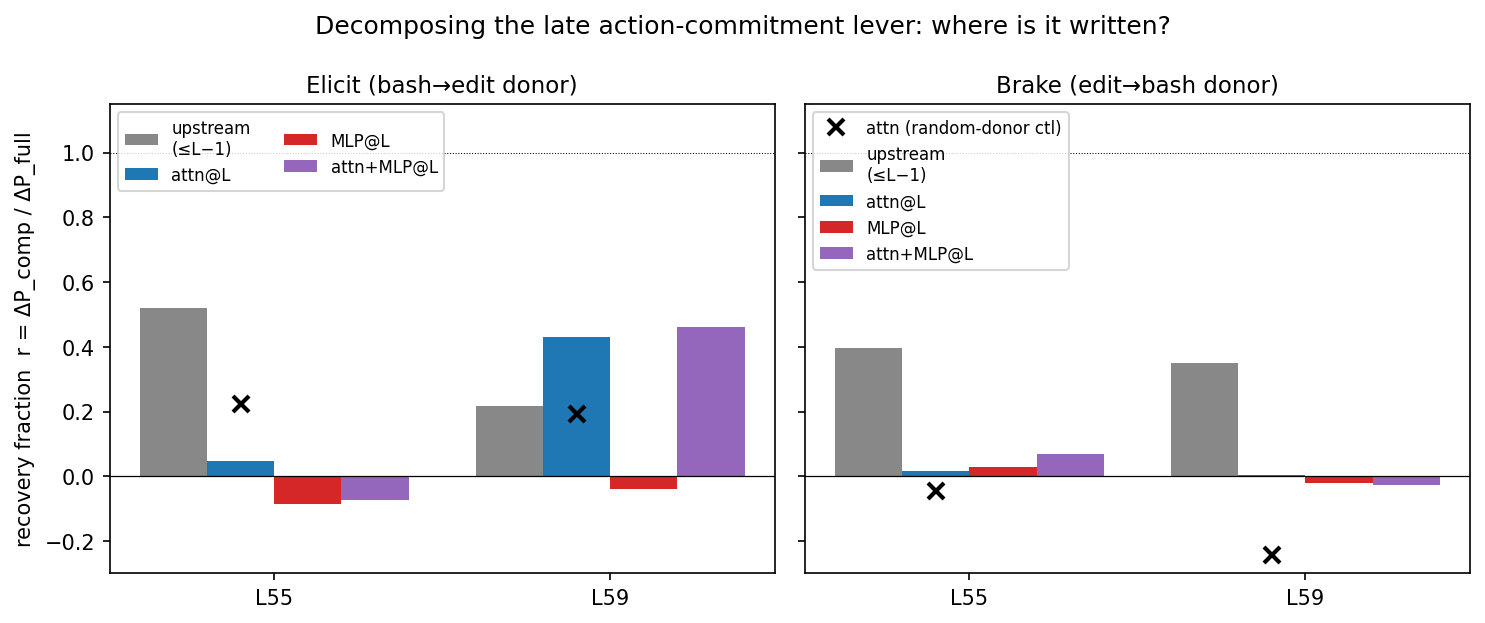
\includegraphics[width=0.82\textwidth]{figures/fig_decomp_attn_mlp.png}
\caption{Component recovery of the late lever. Elicit (left) is carried at L59 by the attention sublayer
(blue), MLP (red) null; brake (right) by neither sublayer. The MLP is inert in all four cells.}
\label{fig:decomp}
\end{figure}

\paragraph{The elicit is a sparse three-head push circuit.}
L59 is a full-attention layer in Qwen3.6's hybrid linear/full stack (every fourth layer is softmax attention),
with 24 query heads. The attention output is again an exact sum over heads, $a_L=\sum_h c_h$ with
$c_h = z_h W_O^{(h)}$~\cite{mathframework}, so we re-inject each head's donor$\to$point difference $\Delta c_h$
alone (head-split reconstruction relative error $0.0015$). The result is \emph{sparse}: heads $8,6,3$ carry
$+0.122,+0.119,+0.083$ while the rest are $\approx 0$ or negative, and the top three together
($\Delta P{=}{+}0.262$) \emph{exceed} all 24 heads jointly ($+0.224$) because an opposing set ($16,19,21,\dots$,
each $-0.01$ to $-0.03$) partially cancels them --- a small push--pull circuit, not a diffuse sum
(Figure~\ref{fig:heads}). Behaviorally the three heads alone lift emission $0.23\!\to\!0.42$ --- $89\%$ of the
all-24-heads rate ($0.47$) and near the attention channel's $0.45$ --- and they are direction-specific (head 8
task-matched $+0.121$ vs.\ cross-repo $+0.077$). Geometric write-magnitude \emph{misleads}: the largest writer along the attention direction (head 21,
projection $14.0$) is causally an \emph{opponent} ($-0.014$) --- only the patch tells the truth. The brake,
re-scanned per head, has \emph{no} head locus and is not a cancellation either (all 24 heads in $[-0.005,+0.012]$),
so the elicit/brake asymmetry holds all the way down to head resolution.

\begin{table}[h]\centering\small
\begin{tabular}{lccc}
\toprule
head set (L59, elicit) & \#heads & $\Delta P(\text{edit})$ & edit-emit \\
\midrule
top-1 $\{8\}$ & 1 & $+0.121$ & --- \\
\textbf{top-3} $\{8,6,3\}$ & 3 & $\mathbf{+0.262}$ & $\mathbf{0.42}$ \\
all heads & 24 & $+0.224$ & $0.47$ \\
top head, cross-repo donor (ctl) & 1 & $+0.077$ & --- \\
\bottomrule
\end{tabular}
\caption{Cumulative head contribution. Three heads reproduce (and overshoot) the full attention effect; emission
baseline is $0.23$. Top-3 $>$ all-24 because an opposing head set partially cancels the push.}
\label{tab:heads}
\end{table}

\begin{figure}[h]\centering
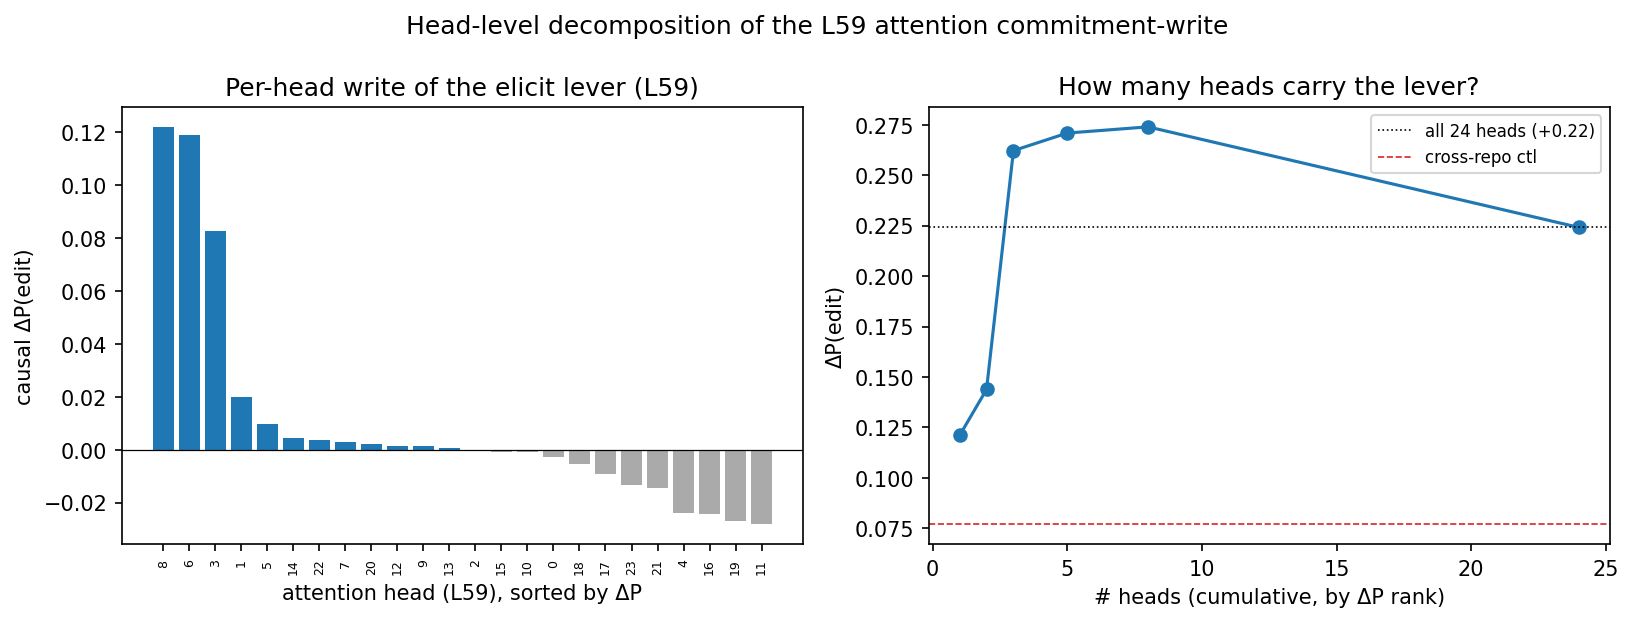
\includegraphics[width=0.82\textwidth]{figures/fig_heads_L59.png}
\caption{Head-level decomposition at L59. Left: per-head causal $\Delta P(\text{edit})$, sorted --- a few heads
push, a few oppose. Right: cumulative recovery; three heads reach (and exceed) the all-heads net.}
\label{fig:heads}
\end{figure}

\paragraph{What the heads read, and a causal source test.}
At the decision token the commit heads attend \emph{globally} (low locality, $\sim$0.10--0.16 of mass in the last
128 keys) to the trajectory's \emph{tool-call history} --- the tool names \texttt{bash} and
\texttt{str\_replace\_editor} and the call's JSON scaffold --- not to any semantic ``task done'' verdict. This is
the attention signature of an induction/copy mechanism~\cite{induction}: the late decision promotes a tool name
from the pattern of prior calls. We tested necessity by ablation~\cite{ioi}. The ideal head-edge knockout (recomputing $o_h=a_h V_h$) is
blocked here: Qwen3.6's full attention is \emph{output-gated} ($z_h = g_h\!\odot\!(a_h V_h)$; the ungated
reconstruction fails, relerr $1.7$--$2.4$), so we instead ablate the \emph{source content}, mean-patching the L59
key/value at the tool-name positions. The agent's tool choice is then causally specific to each tool's name
tokens: ablating \texttt{bash} tokens drops $P(\texttt{bash})$ by $-0.071$ ($-18\%$ relative) versus $-0.000$ for
random, count-matched positions; ablating \texttt{str\_replace\_editor} tokens lowers $P(\text{edit})$ and raises
$P(\texttt{bash})$. Honestly, the edit side is \emph{ceiling-confounded} --- the rows that contain
\texttt{str\_replace\_editor} tokens are already edit-saturated ($P\!\approx\!0.9$), so its drop is small
($-0.031$) --- and this ablation is over all heads, not head-specific. The copy reading is therefore
\emph{supported, not nailed}; a gate-aware head-edge knockout is the named next step.

\paragraph{Synthesis.} Four levels down, the late action-commitment lever resolves to a concrete, sparse circuit:
a handful of induction-style attention heads in a single late full-attention layer (L59) that read the
trajectory's tool-call history and promote a tool name, partially opposed by a counter-set --- not a feed-forward
feature and not an attention to a semantic verdict. The brake, by contrast, has no sublayer and no head locus: it
is a distributed, super-additive residual effect. The agent decides whether to commit an action largely by
\emph{copying the pattern of tools it has already used}.

%==================================================================================================
% Bibliography entries to append to \begin{thebibliography} of the main paper:
%
% \bibitem{geva} M.~Geva, R.~Schuster, J.~Berant, O.~Levy. Transformer Feed-Forward Layers Are Key-Value
%   Memories. EMNLP 2021. arXiv:2012.14913.
% \bibitem{mathframework} N.~Elhage, N.~Nanda, C.~Olsson, et al. A Mathematical Framework for Transformer
%   Circuits. Anthropic, 2021.
% \bibitem{induction} C.~Olsson, N.~Elhage, N.~Nanda, et al. In-context Learning and Induction Heads.
%   Anthropic, 2022. arXiv:2209.11895.
% \bibitem{ioi} K.~Wang, A.~Variengien, A.~Conmy, B.~Shlegeris, J.~Steinhardt. Interpretability in the Wild: a
%   Circuit for Indirect Object Identification in GPT-2 Small. ICLR 2023. arXiv:2211.00593.
 after \S\ref{sec:xmodel} (cross-architecture), before Discussion.
% Requires bib keys: geva, induction, mathframework, ioi (entries listed at the end of this file).

\section{Opening the lever: a sparse attention-head circuit}\label{sec:decomp}
The lever is a single late-layer residual patch; we now open it. Because a pre-norm block writes its output as
an \emph{exact} sum, $y_L = x_L + a_L + m_L$ (input residual, attention contribution, MLP contribution), the
published donor patch $\Delta_{\text{full}} = y^{\text{donor}}_L - y^{\text{point}}_L = \Delta x + \Delta a +
\Delta m$ is exactly additive in the residual. We therefore re-inject each component alone with an additive hook
at the layer-$L$ output and read the one-token $\Delta P(\text{edit})$, the same metric as the dense profile of
\S\ref{sec:stats}. Two gates hold throughout: the additive split reconstructs the captured residual to relative
error $0.0025$ (L55) / $0.0024$ (L59), and the \texttt{full} re-injection reproduces the published lever exactly
(elicit emission $0.23\!\to\!0.77$@L59, brake $0.48\!\to\!0.03$@L55), so the decomposition measures the same
intervention. All numbers are $n{=}60$/condition on Qwen3.6-27B.

\paragraph{Attention writes the elicit; the MLP is inert; the brake is distributed.}
Table~\ref{tab:decomp} gives the recovery fraction $r = \Delta P_{\text{comp}}/\Delta P_{\text{full}}$ of each
component. The two directions decompose \emph{differently}. For the \textbf{elicit}, the L59 attention sublayer
is the single largest writer ($r_{\text{attn}}{=}0.43$, 95\% CI $[0.33,0.53]$), the \textbf{MLP is null}
($r_{\text{mlp}}{=}{-}0.04$; paired Wilcoxon attn$\gg$mlp $p{=}1.8\mathrm{e}{-}8$), and the attention write is
\emph{direction-specific} (task-matched $\Delta P{=}{+}0.223$ vs.\ random-donor $+0.100$, $2.2\times$); under
generation the attention component alone roughly doubles emission ($0.23\!\to\!0.45$) while the MLP component is
inert ($0.25$). At L55 neither sublayer writes the signal --- it is still \emph{arriving} via the residual from
below ($r_{\text{inp}}{=}0.52$) --- so the attention write fires specifically at L59. The \textbf{brake} localizes
to \emph{neither} sublayer ($r_{\text{attn}},r_{\text{mlp}}\!\approx\!0$ at both layers); $\sim$35--40\% is
carried by the upstream residual and the remainder by a large negative \emph{nonlinear interaction} (the gap
$\Delta P_{\text{full}}-\sum\Delta P_{\text{comp}}$ is $-0.23$/$-0.26$). The MLP is null in all four cells. This
rules out a Geva-style feed-forward ``emit-action'' key--value write~\cite{geva}: the late commitment is an
attention/residual phenomenon, and the elicit/brake asymmetry --- attention-written push vs.\ distributed,
irreducible suppression --- holds at sublayer resolution (Figure~\ref{fig:decomp}). The strict pre-registered
threshold ($r_{\text{attn}}{\ge}0.5$) is not met, so we state it honestly: the elicit is attention-\emph{dominated}
but not attention-\emph{sufficient}.

\begin{table}[h]\centering\small
\begin{tabular}{llcccc}
\toprule
direction & layer & $\Delta P_{\text{full}}$ & $r_{\text{inp}}$ & $r_{\text{attn}}$ & $r_{\text{mlp}}$ \\
\midrule
elicit & L55 & $+0.319$ & $0.52$ & $0.05$ & $-0.09$ \\
\textbf{elicit} & \textbf{L59} & $+0.518$ & $0.22$ & $\mathbf{0.43}$ & $-0.04$ \\
brake & L55 & $-0.404$ & $0.40$ & $0.02$ & $0.03$ \\
brake & L59 & $-0.382$ & $0.35$ & $0.00$ & $-0.02$ \\
\bottomrule
\end{tabular}
\caption{Attn-vs-MLP decomposition (recovery fraction $r=\Delta P_{\text{comp}}/\Delta P_{\text{full}}$). The
elicit is attention-written at L59 (MLP null, direction-specific); the brake localizes to no sublayer.}
\label{tab:decomp}
\end{table}

\begin{figure}[h]\centering
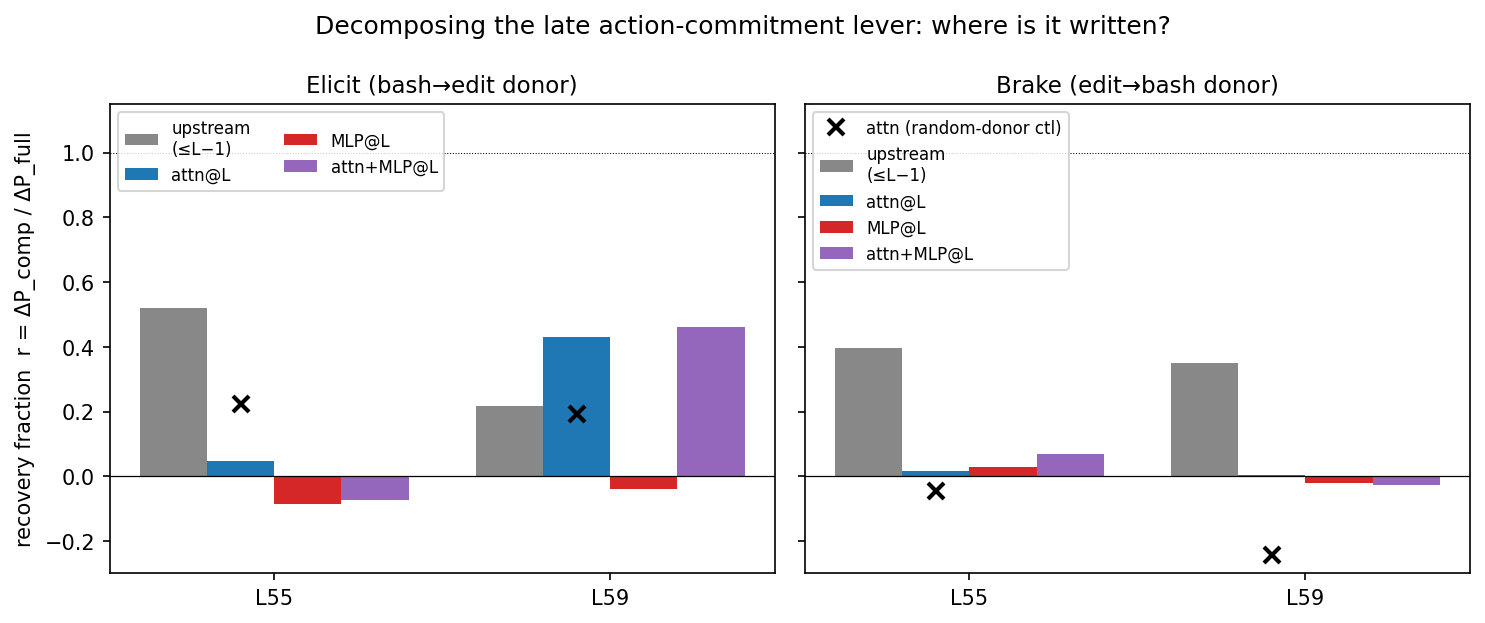
\includegraphics[width=0.82\textwidth]{figures/fig_decomp_attn_mlp.png}
\caption{Component recovery of the late lever. Elicit (left) is carried at L59 by the attention sublayer
(blue), MLP (red) null; brake (right) by neither sublayer. The MLP is inert in all four cells.}
\label{fig:decomp}
\end{figure}

\paragraph{The elicit is a sparse three-head push circuit.}
L59 is a full-attention layer in Qwen3.6's hybrid linear/full stack (every fourth layer is softmax attention),
with 24 query heads. The attention output is again an exact sum over heads, $a_L=\sum_h c_h$ with
$c_h = z_h W_O^{(h)}$~\cite{mathframework}, so we re-inject each head's donor$\to$point difference $\Delta c_h$
alone (head-split reconstruction relative error $0.0015$). The result is \emph{sparse}: heads $8,6,3$ carry
$+0.122,+0.119,+0.083$ while the rest are $\approx 0$ or negative, and the top three together
($\Delta P{=}{+}0.262$) \emph{exceed} all 24 heads jointly ($+0.224$) because an opposing set ($16,19,21,\dots$,
each $-0.01$ to $-0.03$) partially cancels them --- a small push--pull circuit, not a diffuse sum
(Figure~\ref{fig:heads}). Behaviorally the three heads alone lift emission $0.23\!\to\!0.42$ --- $89\%$ of the
all-24-heads rate ($0.47$) and near the attention channel's $0.45$ --- and they are direction-specific (head 8
task-matched $+0.121$ vs.\ cross-repo $+0.077$). Geometric write-magnitude \emph{misleads}: the largest writer along the attention direction (head 21,
projection $14.0$) is causally an \emph{opponent} ($-0.014$) --- only the patch tells the truth. The brake,
re-scanned per head, has \emph{no} head locus and is not a cancellation either (all 24 heads in $[-0.005,+0.012]$),
so the elicit/brake asymmetry holds all the way down to head resolution.

\begin{table}[h]\centering\small
\begin{tabular}{lccc}
\toprule
head set (L59, elicit) & \#heads & $\Delta P(\text{edit})$ & edit-emit \\
\midrule
top-1 $\{8\}$ & 1 & $+0.121$ & --- \\
\textbf{top-3} $\{8,6,3\}$ & 3 & $\mathbf{+0.262}$ & $\mathbf{0.42}$ \\
all heads & 24 & $+0.224$ & $0.47$ \\
top head, cross-repo donor (ctl) & 1 & $+0.077$ & --- \\
\bottomrule
\end{tabular}
\caption{Cumulative head contribution. Three heads reproduce (and overshoot) the full attention effect; emission
baseline is $0.23$. Top-3 $>$ all-24 because an opposing head set partially cancels the push.}
\label{tab:heads}
\end{table}

\begin{figure}[h]\centering
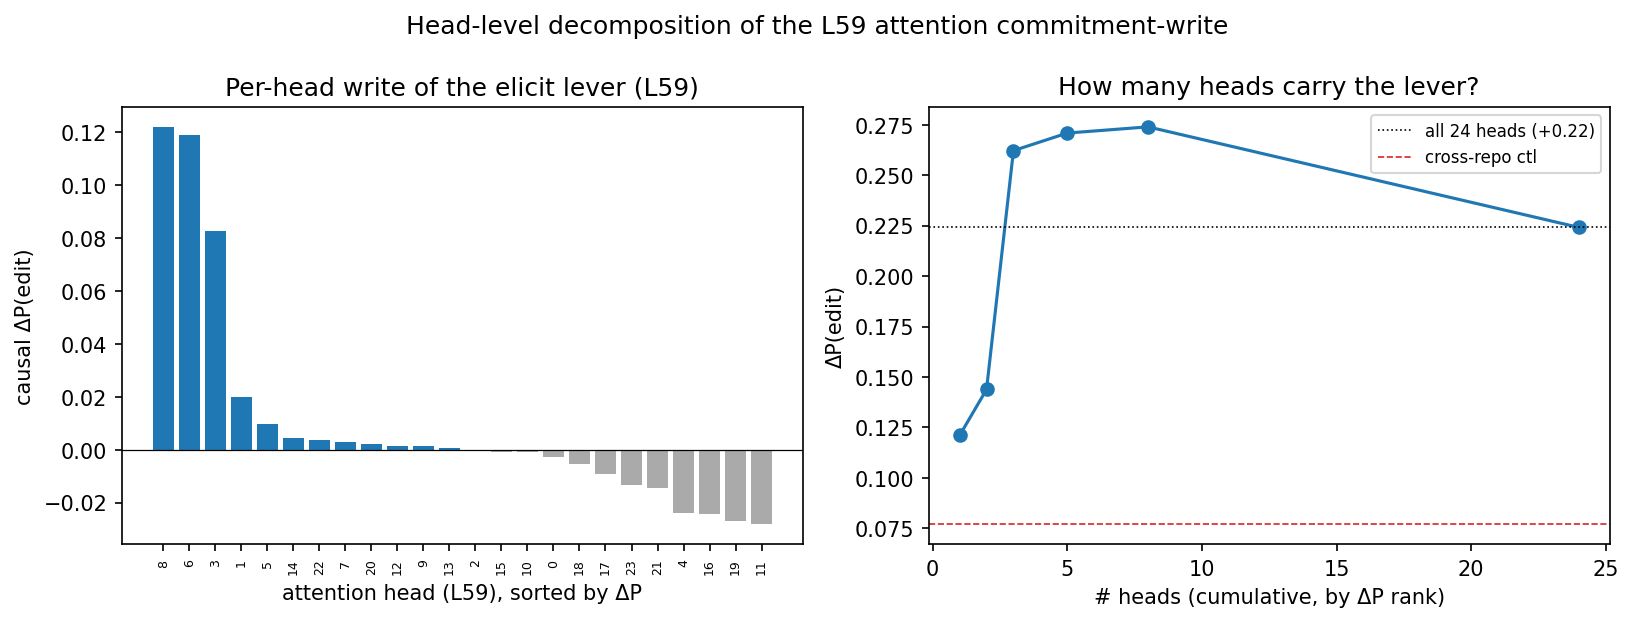
\includegraphics[width=0.82\textwidth]{figures/fig_heads_L59.png}
\caption{Head-level decomposition at L59. Left: per-head causal $\Delta P(\text{edit})$, sorted --- a few heads
push, a few oppose. Right: cumulative recovery; three heads reach (and exceed) the all-heads net.}
\label{fig:heads}
\end{figure}

\paragraph{What the heads read, and a causal source test.}
At the decision token the commit heads attend \emph{globally} (low locality, $\sim$0.10--0.16 of mass in the last
128 keys) to the trajectory's \emph{tool-call history} --- the tool names \texttt{bash} and
\texttt{str\_replace\_editor} and the call's JSON scaffold --- not to any semantic ``task done'' verdict. This is
the attention signature of an induction/copy mechanism~\cite{induction}: the late decision promotes a tool name
from the pattern of prior calls. We tested necessity by ablation~\cite{ioi}. The ideal head-edge knockout (recomputing $o_h=a_h V_h$) is
blocked here: Qwen3.6's full attention is \emph{output-gated} ($z_h = g_h\!\odot\!(a_h V_h)$; the ungated
reconstruction fails, relerr $1.7$--$2.4$), so we instead ablate the \emph{source content}, mean-patching the L59
key/value at the tool-name positions. The agent's tool choice is then causally specific to each tool's name
tokens: ablating \texttt{bash} tokens drops $P(\texttt{bash})$ by $-0.071$ ($-18\%$ relative) versus $-0.000$ for
random, count-matched positions; ablating \texttt{str\_replace\_editor} tokens lowers $P(\text{edit})$ and raises
$P(\texttt{bash})$. Honestly, the edit side is \emph{ceiling-confounded} --- the rows that contain
\texttt{str\_replace\_editor} tokens are already edit-saturated ($P\!\approx\!0.9$), so its drop is small
($-0.031$) --- and this ablation is over all heads, not head-specific. The copy reading is therefore
\emph{supported, not nailed}; a gate-aware head-edge knockout is the named next step.

\paragraph{Synthesis.} Four levels down, the late action-commitment lever resolves to a concrete, sparse circuit:
a handful of induction-style attention heads in a single late full-attention layer (L59) that read the
trajectory's tool-call history and promote a tool name, partially opposed by a counter-set --- not a feed-forward
feature and not an attention to a semantic verdict. The brake, by contrast, has no sublayer and no head locus: it
is a distributed, super-additive residual effect. The agent decides whether to commit an action largely by
\emph{copying the pattern of tools it has already used}.

%==================================================================================================
% Bibliography entries to append to \begin{thebibliography} of the main paper:
%
% \bibitem{geva} M.~Geva, R.~Schuster, J.~Berant, O.~Levy. Transformer Feed-Forward Layers Are Key-Value
%   Memories. EMNLP 2021. arXiv:2012.14913.
% \bibitem{mathframework} N.~Elhage, N.~Nanda, C.~Olsson, et al. A Mathematical Framework for Transformer
%   Circuits. Anthropic, 2021.
% \bibitem{induction} C.~Olsson, N.~Elhage, N.~Nanda, et al. In-context Learning and Induction Heads.
%   Anthropic, 2022. arXiv:2209.11895.
% \bibitem{ioi} K.~Wang, A.~Variengien, A.~Conmy, B.~Shlegeris, J.~Steinhardt. Interpretability in the Wild: a
%   Circuit for Indirect Object Identification in GPT-2 Small. ICLR 2023. arXiv:2211.00593.
 after \S\ref{sec:xmodel} (cross-architecture), before Discussion.
% Requires bib keys: geva, induction, mathframework, ioi (entries listed at the end of this file).

\section{Opening the lever: a sparse attention-head circuit}\label{sec:decomp}
The lever is a single late-layer residual patch; we now open it. Because a pre-norm block writes its output as
an \emph{exact} sum, $y_L = x_L + a_L + m_L$ (input residual, attention contribution, MLP contribution), the
published donor patch $\Delta_{\text{full}} = y^{\text{donor}}_L - y^{\text{point}}_L = \Delta x + \Delta a +
\Delta m$ is exactly additive in the residual. We therefore re-inject each component alone with an additive hook
at the layer-$L$ output and read the one-token $\Delta P(\text{edit})$, the same metric as the dense profile of
\S\ref{sec:stats}. Two gates hold throughout: the additive split reconstructs the captured residual to relative
error $0.0025$ (L55) / $0.0024$ (L59), and the \texttt{full} re-injection reproduces the published lever exactly
(elicit emission $0.23\!\to\!0.77$@L59, brake $0.48\!\to\!0.03$@L55), so the decomposition measures the same
intervention. All numbers are $n{=}60$/condition on Qwen3.6-27B.

\paragraph{Attention writes the elicit; the MLP is inert; the brake is distributed.}
Table~\ref{tab:decomp} gives the recovery fraction $r = \Delta P_{\text{comp}}/\Delta P_{\text{full}}$ of each
component. The two directions decompose \emph{differently}. For the \textbf{elicit}, the L59 attention sublayer
is the single largest writer ($r_{\text{attn}}{=}0.43$, 95\% CI $[0.33,0.53]$), the \textbf{MLP is null}
($r_{\text{mlp}}{=}{-}0.04$; paired Wilcoxon attn$\gg$mlp $p{=}1.8\mathrm{e}{-}8$), and the attention write is
\emph{direction-specific} (task-matched $\Delta P{=}{+}0.223$ vs.\ random-donor $+0.100$, $2.2\times$); under
generation the attention component alone roughly doubles emission ($0.23\!\to\!0.45$) while the MLP component is
inert ($0.25$). At L55 neither sublayer writes the signal --- it is still \emph{arriving} via the residual from
below ($r_{\text{inp}}{=}0.52$) --- so the attention write fires specifically at L59. The \textbf{brake} localizes
to \emph{neither} sublayer ($r_{\text{attn}},r_{\text{mlp}}\!\approx\!0$ at both layers); $\sim$35--40\% is
carried by the upstream residual and the remainder by a large negative \emph{nonlinear interaction} (the gap
$\Delta P_{\text{full}}-\sum\Delta P_{\text{comp}}$ is $-0.23$/$-0.26$). The MLP is null in all four cells. This
rules out a Geva-style feed-forward ``emit-action'' key--value write~\cite{geva}: the late commitment is an
attention/residual phenomenon, and the elicit/brake asymmetry --- attention-written push vs.\ distributed,
irreducible suppression --- holds at sublayer resolution (Figure~\ref{fig:decomp}). The strict pre-registered
threshold ($r_{\text{attn}}{\ge}0.5$) is not met, so we state it honestly: the elicit is attention-\emph{dominated}
but not attention-\emph{sufficient}.

\begin{table}[h]\centering\small
\begin{tabular}{llcccc}
\toprule
direction & layer & $\Delta P_{\text{full}}$ & $r_{\text{inp}}$ & $r_{\text{attn}}$ & $r_{\text{mlp}}$ \\
\midrule
elicit & L55 & $+0.319$ & $0.52$ & $0.05$ & $-0.09$ \\
\textbf{elicit} & \textbf{L59} & $+0.518$ & $0.22$ & $\mathbf{0.43}$ & $-0.04$ \\
brake & L55 & $-0.404$ & $0.40$ & $0.02$ & $0.03$ \\
brake & L59 & $-0.382$ & $0.35$ & $0.00$ & $-0.02$ \\
\bottomrule
\end{tabular}
\caption{Attn-vs-MLP decomposition (recovery fraction $r=\Delta P_{\text{comp}}/\Delta P_{\text{full}}$). The
elicit is attention-written at L59 (MLP null, direction-specific); the brake localizes to no sublayer.}
\label{tab:decomp}
\end{table}

\begin{figure}[h]\centering
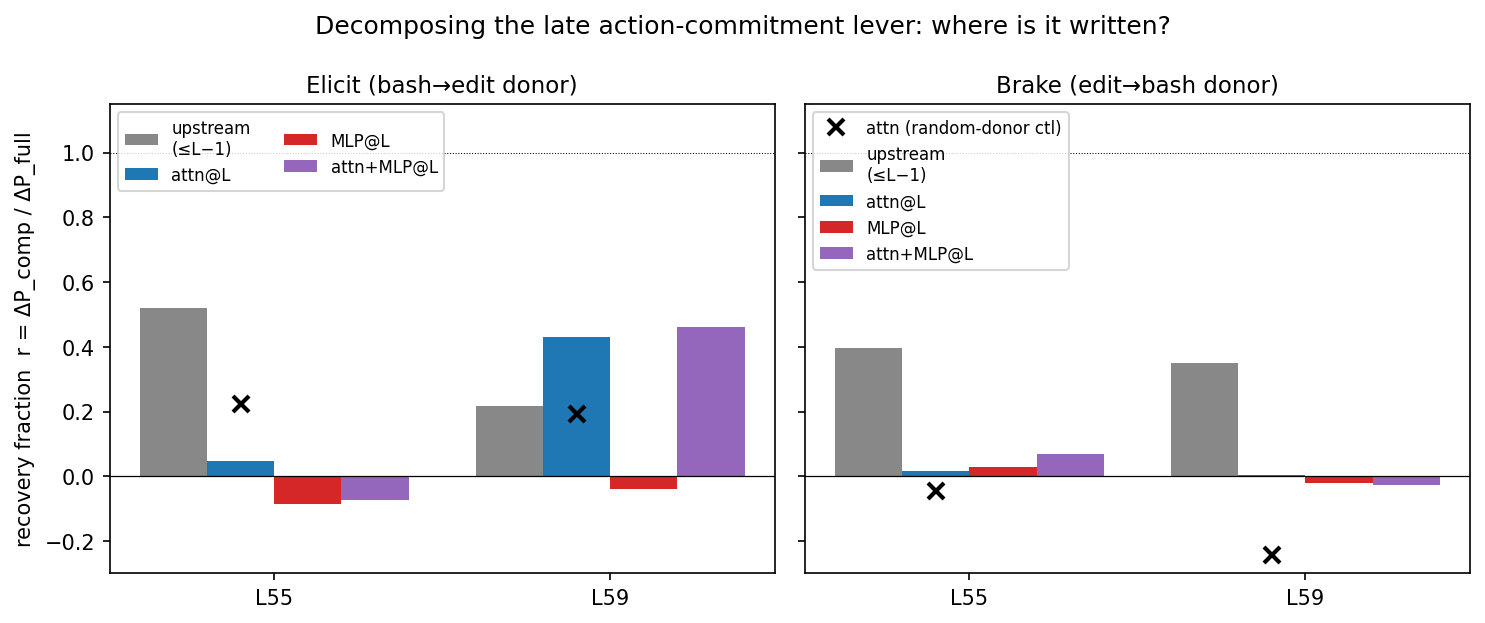
\includegraphics[width=0.82\textwidth]{figures/fig_decomp_attn_mlp.png}
\caption{Component recovery of the late lever. Elicit (left) is carried at L59 by the attention sublayer
(blue), MLP (red) null; brake (right) by neither sublayer. The MLP is inert in all four cells.}
\label{fig:decomp}
\end{figure}

\paragraph{The elicit is a sparse three-head push circuit.}
L59 is a full-attention layer in Qwen3.6's hybrid linear/full stack (every fourth layer is softmax attention),
with 24 query heads. The attention output is again an exact sum over heads, $a_L=\sum_h c_h$ with
$c_h = z_h W_O^{(h)}$~\cite{mathframework}, so we re-inject each head's donor$\to$point difference $\Delta c_h$
alone (head-split reconstruction relative error $0.0015$). The result is \emph{sparse}: heads $8,6,3$ carry
$+0.122,+0.119,+0.083$ while the rest are $\approx 0$ or negative, and the top three together
($\Delta P{=}{+}0.262$) \emph{exceed} all 24 heads jointly ($+0.224$) because an opposing set ($16,19,21,\dots$,
each $-0.01$ to $-0.03$) partially cancels them --- a small push--pull circuit, not a diffuse sum
(Figure~\ref{fig:heads}). Behaviorally the three heads alone lift emission $0.23\!\to\!0.42$ --- $89\%$ of the
all-24-heads rate ($0.47$) and near the attention channel's $0.45$ --- and they are direction-specific (head 8
task-matched $+0.121$ vs.\ cross-repo $+0.077$). Geometric write-magnitude \emph{misleads}: the largest writer along the attention direction (head 21,
projection $14.0$) is causally an \emph{opponent} ($-0.014$) --- only the patch tells the truth. The brake,
re-scanned per head, has \emph{no} head locus and is not a cancellation either (all 24 heads in $[-0.005,+0.012]$),
so the elicit/brake asymmetry holds all the way down to head resolution.

\begin{table}[h]\centering\small
\begin{tabular}{lccc}
\toprule
head set (L59, elicit) & \#heads & $\Delta P(\text{edit})$ & edit-emit \\
\midrule
top-1 $\{8\}$ & 1 & $+0.121$ & --- \\
\textbf{top-3} $\{8,6,3\}$ & 3 & $\mathbf{+0.262}$ & $\mathbf{0.42}$ \\
all heads & 24 & $+0.224$ & $0.47$ \\
top head, cross-repo donor (ctl) & 1 & $+0.077$ & --- \\
\bottomrule
\end{tabular}
\caption{Cumulative head contribution. Three heads reproduce (and overshoot) the full attention effect; emission
baseline is $0.23$. Top-3 $>$ all-24 because an opposing head set partially cancels the push.}
\label{tab:heads}
\end{table}

\begin{figure}[h]\centering
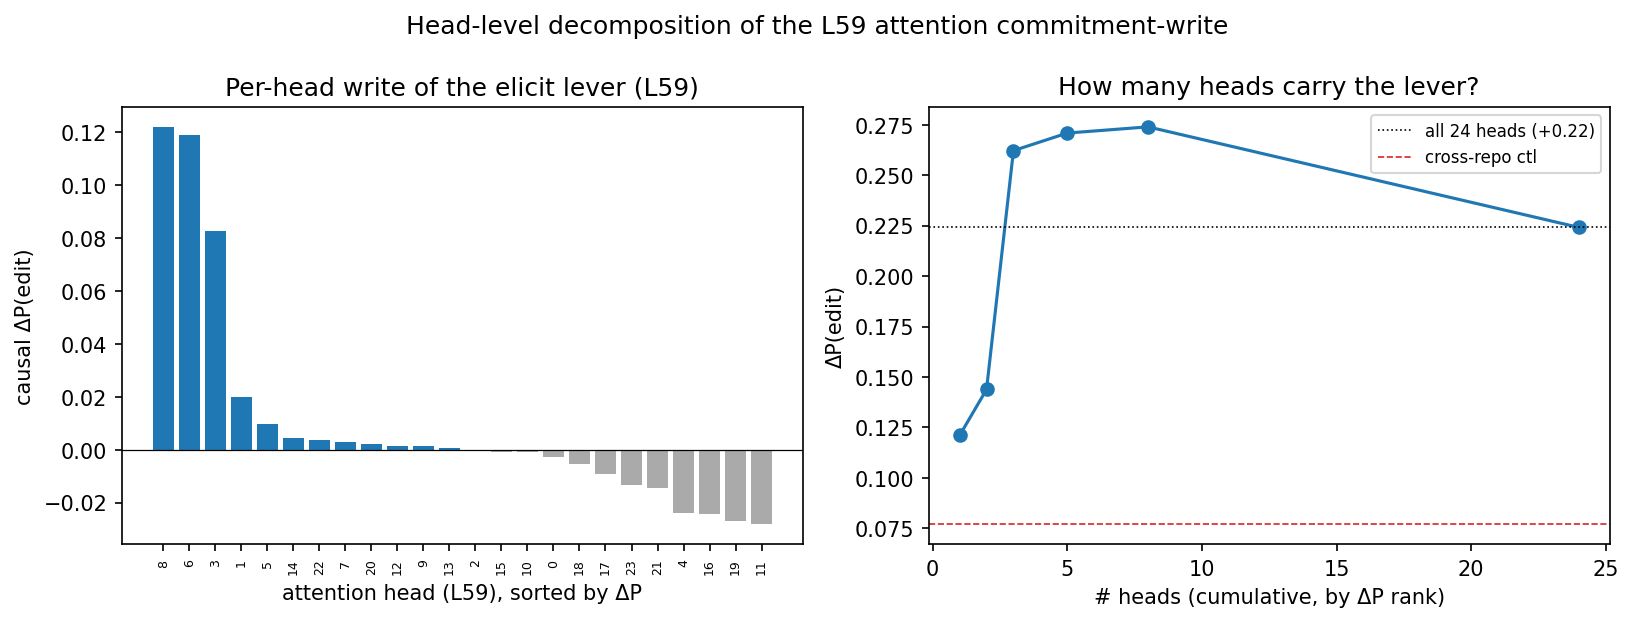
\includegraphics[width=0.82\textwidth]{figures/fig_heads_L59.png}
\caption{Head-level decomposition at L59. Left: per-head causal $\Delta P(\text{edit})$, sorted --- a few heads
push, a few oppose. Right: cumulative recovery; three heads reach (and exceed) the all-heads net.}
\label{fig:heads}
\end{figure}

\paragraph{What the heads read, and a causal source test.}
At the decision token the commit heads attend \emph{globally} (low locality, $\sim$0.10--0.16 of mass in the last
128 keys) to the trajectory's \emph{tool-call history} --- the tool names \texttt{bash} and
\texttt{str\_replace\_editor} and the call's JSON scaffold --- not to any semantic ``task done'' verdict. This is
the attention signature of an induction/copy mechanism~\cite{induction}: the late decision promotes a tool name
from the pattern of prior calls. We tested necessity by ablation~\cite{ioi}. The ideal head-edge knockout (recomputing $o_h=a_h V_h$) is
blocked here: Qwen3.6's full attention is \emph{output-gated} ($z_h = g_h\!\odot\!(a_h V_h)$; the ungated
reconstruction fails, relerr $1.7$--$2.4$), so we instead ablate the \emph{source content}, mean-patching the L59
key/value at the tool-name positions. The agent's tool choice is then causally specific to each tool's name
tokens: ablating \texttt{bash} tokens drops $P(\texttt{bash})$ by $-0.071$ ($-18\%$ relative) versus $-0.000$ for
random, count-matched positions; ablating \texttt{str\_replace\_editor} tokens lowers $P(\text{edit})$ and raises
$P(\texttt{bash})$. Honestly, the edit side is \emph{ceiling-confounded} --- the rows that contain
\texttt{str\_replace\_editor} tokens are already edit-saturated ($P\!\approx\!0.9$), so its drop is small
($-0.031$) --- and this ablation is over all heads, not head-specific. The copy reading is therefore
\emph{supported, not nailed}; a gate-aware head-edge knockout is the named next step.

\paragraph{Synthesis.} Four levels down, the late action-commitment lever resolves to a concrete, sparse circuit:
a handful of induction-style attention heads in a single late full-attention layer (L59) that read the
trajectory's tool-call history and promote a tool name, partially opposed by a counter-set --- not a feed-forward
feature and not an attention to a semantic verdict. The brake, by contrast, has no sublayer and no head locus: it
is a distributed, super-additive residual effect. The agent decides whether to commit an action largely by
\emph{copying the pattern of tools it has already used}.

%==================================================================================================
% Bibliography entries to append to \begin{thebibliography} of the main paper:
%
% \bibitem{geva} M.~Geva, R.~Schuster, J.~Berant, O.~Levy. Transformer Feed-Forward Layers Are Key-Value
%   Memories. EMNLP 2021. arXiv:2012.14913.
% \bibitem{mathframework} N.~Elhage, N.~Nanda, C.~Olsson, et al. A Mathematical Framework for Transformer
%   Circuits. Anthropic, 2021.
% \bibitem{induction} C.~Olsson, N.~Elhage, N.~Nanda, et al. In-context Learning and Induction Heads.
%   Anthropic, 2022. arXiv:2209.11895.
% \bibitem{ioi} K.~Wang, A.~Variengien, A.~Conmy, B.~Shlegeris, J.~Steinhardt. Interpretability in the Wild: a
%   Circuit for Indirect Object Identification in GPT-2 Small. ICLR 2023. arXiv:2211.00593.
 after \S\ref{sec:xmodel} (cross-architecture), before Discussion.
% Requires bib keys: geva, induction, mathframework, ioi (entries listed at the end of this file).

\section{Opening the lever: a sparse attention-head circuit}\label{sec:decomp}
The lever is a single late-layer residual patch; we now open it. Because a pre-norm block writes its output as
an \emph{exact} sum, $y_L = x_L + a_L + m_L$ (input residual, attention contribution, MLP contribution), the
published donor patch $\Delta_{\text{full}} = y^{\text{donor}}_L - y^{\text{point}}_L = \Delta x + \Delta a +
\Delta m$ is exactly additive in the residual. We therefore re-inject each component alone with an additive hook
at the layer-$L$ output and read the one-token $\Delta P(\text{edit})$, the same metric as the dense profile of
\S\ref{sec:stats}. Two gates hold throughout: the additive split reconstructs the captured residual to relative
error $0.0025$ (L55) / $0.0024$ (L59), and the \texttt{full} re-injection reproduces the published lever exactly
(elicit emission $0.23\!\to\!0.77$@L59, brake $0.48\!\to\!0.03$@L55), so the decomposition measures the same
intervention. All numbers are $n{=}60$/condition on Qwen3.6-27B.

\paragraph{Attention writes the elicit; the MLP is inert; the brake is distributed.}
Table~\ref{tab:decomp} gives the recovery fraction $r = \Delta P_{\text{comp}}/\Delta P_{\text{full}}$ of each
component. The two directions decompose \emph{differently}. For the \textbf{elicit}, the L59 attention sublayer
is the single largest writer ($r_{\text{attn}}{=}0.43$, 95\% CI $[0.33,0.53]$), the \textbf{MLP is null}
($r_{\text{mlp}}{=}{-}0.04$; paired Wilcoxon attn$\gg$mlp $p{=}1.8\mathrm{e}{-}8$), and the attention write is
\emph{direction-specific} (task-matched $\Delta P{=}{+}0.223$ vs.\ random-donor $+0.100$, $2.2\times$); under
generation the attention component alone roughly doubles emission ($0.23\!\to\!0.45$) while the MLP component is
inert ($0.25$). At L55 neither sublayer writes the signal --- it is still \emph{arriving} via the residual from
below ($r_{\text{inp}}{=}0.52$) --- so the attention write fires specifically at L59. The \textbf{brake} localizes
to \emph{neither} sublayer ($r_{\text{attn}},r_{\text{mlp}}\!\approx\!0$ at both layers); $\sim$35--40\% is
carried by the upstream residual and the remainder by a large negative \emph{nonlinear interaction} (the gap
$\Delta P_{\text{full}}-\sum\Delta P_{\text{comp}}$ is $-0.23$/$-0.26$). The MLP is null in all four cells. This
rules out a Geva-style feed-forward ``emit-action'' key--value write~\cite{geva}: the late commitment is an
attention/residual phenomenon, and the elicit/brake asymmetry --- attention-written push vs.\ distributed,
irreducible suppression --- holds at sublayer resolution (Figure~\ref{fig:decomp}). The strict pre-registered
threshold ($r_{\text{attn}}{\ge}0.5$) is not met, so we state it honestly: the elicit is attention-\emph{dominated}
but not attention-\emph{sufficient}.

\begin{table}[h]\centering\small
\begin{tabular}{llcccc}
\toprule
direction & layer & $\Delta P_{\text{full}}$ & $r_{\text{inp}}$ & $r_{\text{attn}}$ & $r_{\text{mlp}}$ \\
\midrule
elicit & L55 & $+0.319$ & $0.52$ & $0.05$ & $-0.09$ \\
\textbf{elicit} & \textbf{L59} & $+0.518$ & $0.22$ & $\mathbf{0.43}$ & $-0.04$ \\
brake & L55 & $-0.404$ & $0.40$ & $0.02$ & $0.03$ \\
brake & L59 & $-0.382$ & $0.35$ & $0.00$ & $-0.02$ \\
\bottomrule
\end{tabular}
\caption{Attn-vs-MLP decomposition (recovery fraction $r=\Delta P_{\text{comp}}/\Delta P_{\text{full}}$). The
elicit is attention-written at L59 (MLP null, direction-specific); the brake localizes to no sublayer.}
\label{tab:decomp}
\end{table}

\begin{figure}[h]\centering
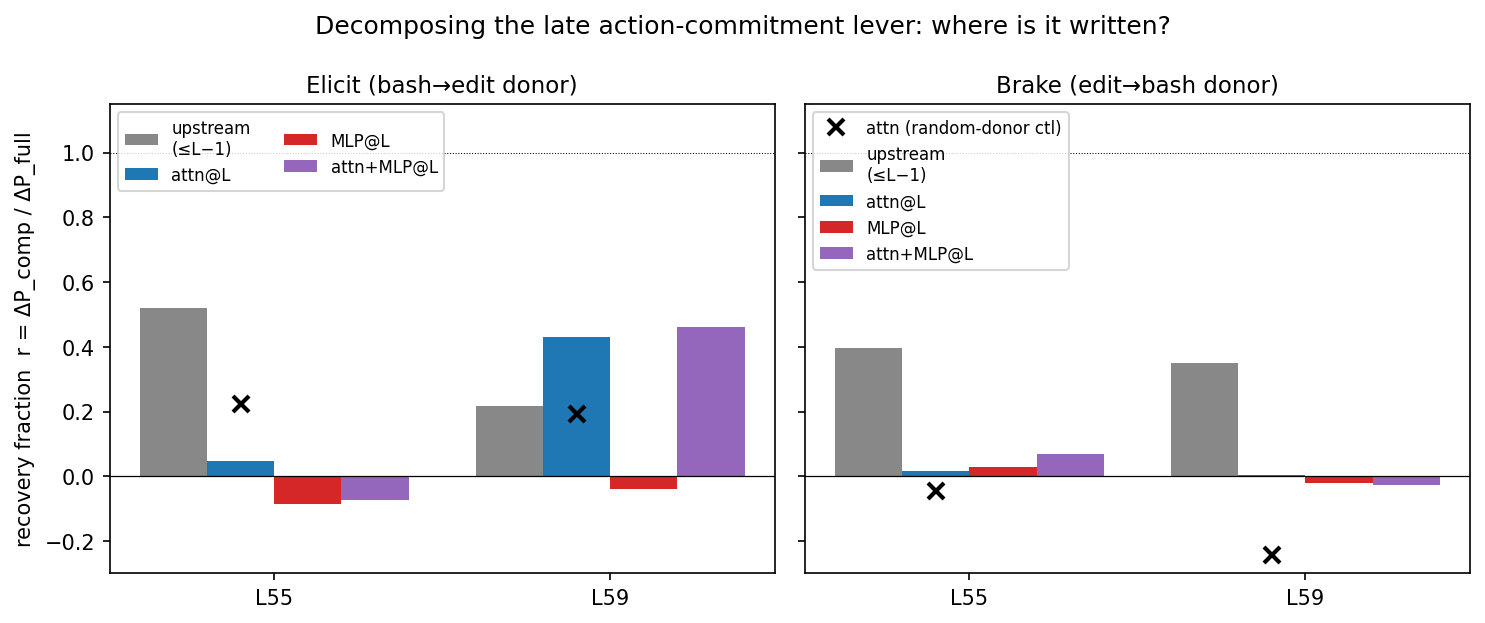
\includegraphics[width=0.82\textwidth]{figures/fig_decomp_attn_mlp.png}
\caption{Component recovery of the late lever. Elicit (left) is carried at L59 by the attention sublayer
(blue), MLP (red) null; brake (right) by neither sublayer. The MLP is inert in all four cells.}
\label{fig:decomp}
\end{figure}

\paragraph{The elicit is a sparse three-head push circuit.}
L59 is a full-attention layer in Qwen3.6's hybrid linear/full stack (every fourth layer is softmax attention),
with 24 query heads. The attention output is again an exact sum over heads, $a_L=\sum_h c_h$ with
$c_h = z_h W_O^{(h)}$~\cite{mathframework}, so we re-inject each head's donor$\to$point difference $\Delta c_h$
alone (head-split reconstruction relative error $0.0015$). The result is \emph{sparse}: heads $8,6,3$ carry
$+0.122,+0.119,+0.083$ while the rest are $\approx 0$ or negative, and the top three together
($\Delta P{=}{+}0.262$) \emph{exceed} all 24 heads jointly ($+0.224$) because an opposing set ($16,19,21,\dots$,
each $-0.01$ to $-0.03$) partially cancels them --- a small push--pull circuit, not a diffuse sum
(Figure~\ref{fig:heads}). Behaviorally the three heads alone lift emission $0.23\!\to\!0.42$ --- $89\%$ of the
all-24-heads rate ($0.47$) and near the attention channel's $0.45$ --- and they are direction-specific (head 8
task-matched $+0.121$ vs.\ cross-repo $+0.077$). Geometric write-magnitude \emph{misleads}: the largest writer along the attention direction (head 21,
projection $14.0$) is causally an \emph{opponent} ($-0.014$) --- only the patch tells the truth. The brake,
re-scanned per head, has \emph{no} head locus and is not a cancellation either (all 24 heads in $[-0.005,+0.012]$),
so the elicit/brake asymmetry holds all the way down to head resolution.

\begin{table}[h]\centering\small
\begin{tabular}{lccc}
\toprule
head set (L59, elicit) & \#heads & $\Delta P(\text{edit})$ & edit-emit \\
\midrule
top-1 $\{8\}$ & 1 & $+0.121$ & --- \\
\textbf{top-3} $\{8,6,3\}$ & 3 & $\mathbf{+0.262}$ & $\mathbf{0.42}$ \\
all heads & 24 & $+0.224$ & $0.47$ \\
top head, cross-repo donor (ctl) & 1 & $+0.077$ & --- \\
\bottomrule
\end{tabular}
\caption{Cumulative head contribution. Three heads reproduce (and overshoot) the full attention effect; emission
baseline is $0.23$. Top-3 $>$ all-24 because an opposing head set partially cancels the push.}
\label{tab:heads}
\end{table}

\begin{figure}[h]\centering
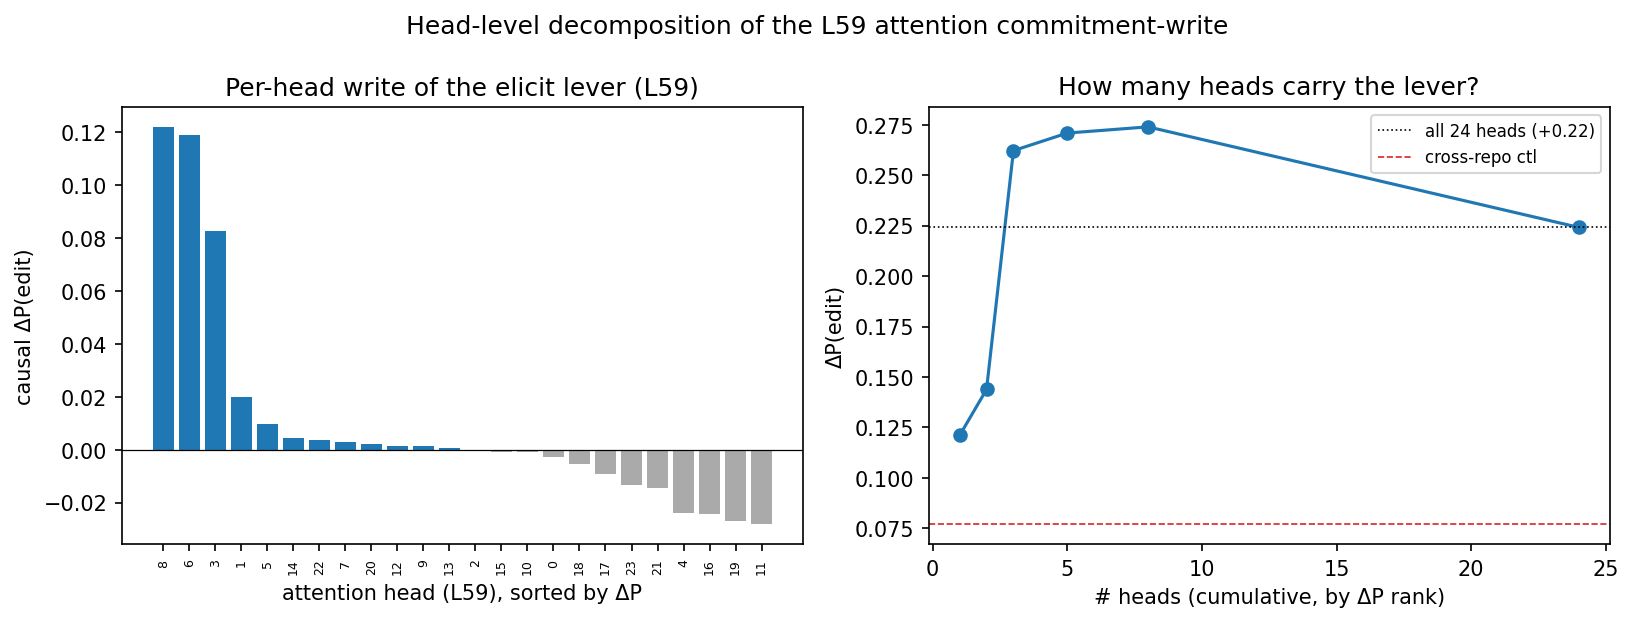
\includegraphics[width=0.82\textwidth]{figures/fig_heads_L59.png}
\caption{Head-level decomposition at L59. Left: per-head causal $\Delta P(\text{edit})$, sorted --- a few heads
push, a few oppose. Right: cumulative recovery; three heads reach (and exceed) the all-heads net.}
\label{fig:heads}
\end{figure}

\paragraph{What the heads read, and a causal source test.}
At the decision token the commit heads attend \emph{globally} (low locality, $\sim$0.10--0.16 of mass in the last
128 keys) to the trajectory's \emph{tool-call history} --- the tool names \texttt{bash} and
\texttt{str\_replace\_editor} and the call's JSON scaffold --- not to any semantic ``task done'' verdict. This is
the attention signature of an induction/copy mechanism~\cite{induction}: the late decision promotes a tool name
from the pattern of prior calls. We tested necessity by ablation~\cite{ioi}. The ideal head-edge knockout (recomputing $o_h=a_h V_h$) is
blocked here: Qwen3.6's full attention is \emph{output-gated} ($z_h = g_h\!\odot\!(a_h V_h)$; the ungated
reconstruction fails, relerr $1.7$--$2.4$), so we instead ablate the \emph{source content}, mean-patching the L59
key/value at the tool-name positions. The agent's tool choice is then causally specific to each tool's name
tokens: ablating \texttt{bash} tokens drops $P(\texttt{bash})$ by $-0.071$ ($-18\%$ relative) versus $-0.000$ for
random, count-matched positions; ablating \texttt{str\_replace\_editor} tokens lowers $P(\text{edit})$ and raises
$P(\texttt{bash})$. Honestly, the edit side is \emph{ceiling-confounded} --- the rows that contain
\texttt{str\_replace\_editor} tokens are already edit-saturated ($P\!\approx\!0.9$), so its drop is small
($-0.031$) --- and this ablation is over all heads, not head-specific. The copy reading is therefore
\emph{supported, not nailed}; a gate-aware head-edge knockout is the named next step.

\paragraph{Synthesis.} Four levels down, the late action-commitment lever resolves to a concrete, sparse circuit:
a handful of induction-style attention heads in a single late full-attention layer (L59) that read the
trajectory's tool-call history and promote a tool name, partially opposed by a counter-set --- not a feed-forward
feature and not an attention to a semantic verdict. The brake, by contrast, has no sublayer and no head locus: it
is a distributed, super-additive residual effect. The agent decides whether to commit an action largely by
\emph{copying the pattern of tools it has already used}.

%==================================================================================================
% Bibliography entries to append to \begin{thebibliography} of the main paper:
%
% \bibitem{geva} M.~Geva, R.~Schuster, J.~Berant, O.~Levy. Transformer Feed-Forward Layers Are Key-Value
%   Memories. EMNLP 2021. arXiv:2012.14913.
% \bibitem{mathframework} N.~Elhage, N.~Nanda, C.~Olsson, et al. A Mathematical Framework for Transformer
%   Circuits. Anthropic, 2021.
% \bibitem{induction} C.~Olsson, N.~Elhage, N.~Nanda, et al. In-context Learning and Induction Heads.
%   Anthropic, 2022. arXiv:2209.11895.
% \bibitem{ioi} K.~Wang, A.~Variengien, A.~Conmy, B.~Shlegeris, J.~Steinhardt. Interpretability in the Wild: a
%   Circuit for Indirect Object Identification in GPT-2 Small. ICLR 2023. arXiv:2211.00593.
